%   % !TEX root = ../../VIII,3_Rahmen-TeX_9-0.tex
%  
%   Signatur/Tex-Datei:	LH_37_05_017
%   RK-Nr. 	60276
%			
%   Titel: 			Si corpus incurrens sistatur, non eadem servatur potentia	
%   Datierung:		Italienaufenthalt (März 1689-März 1690)
%   edlabels:			1
%   Diagramme: 		2 
%
%
%
\selectlanguage{ngerman}
\frenchspacing
%
\begin{ledgroupsized}[r]{120mm}
\footnotesize
\pstart
\noindent\textbf{Überlieferung:}
\pend
\end{ledgroupsized}
%
\begin{ledgroupsized}[r]{114mm}
\footnotesize
\pstart \parindent -6mm
\makebox[6mm][l]{\textit{L}}%
Konzept: LH~XXXVII~5 Bl.~17.
Ein Zettel (ca.~9~x~10,5~cm.);
italienisches Papier;
rechter, linker und unterer Rand beschnitten; Papiererhaltungsmaßnahmen.
Eine Seite auf Bl.~17~r\textsuperscript{o};
Bl.~17~v\textsuperscript{o} leer bis auf ein nicht zuordenbares Zeichen (längliches Kreuz).
\pend
\end{ledgroupsized}
%
%
\vspace{5mm}
\begin{ledgroup}
\footnotesize
\pstart
\noindent%
\textbf{Datierungsgründe:}
Wegen der Verwendung italienischen Papiers kann von einer Abfassung des Konzepts während des Italienaufenthaltes (März 1689 bis März 1690) ausgegangen werden.
%
\pend
%
\pstart
In dem Konzept führt Leibniz ein Gedankenexperiment aus, bei dem kein tatsächlicher Stoß zweier Körper,
%
sondern ein \glqq Quasi-Stoß\grqq, im Mittelpunkt steht: 
%
Die Bahn des \glqq stoßenden\grqq\  und des zunächst ruhenden Körpers fallen nicht auf dieselbe Gerade,
%
sondern werden als zueinander parallel angenommen; 
%
der Weg des Schwerpunkts verläuft, ebenfalls geradlinig, dazwischen.
%
Nichtsdestotrotz scheint das Gedankenexperiment als eine Analogie angedacht zu sein,
%
um mit deren Hilfe über die Erhaltung bzw.\ Nichterhaltung der Kraft im entsprechenden \glqq echten\grqq\ Stoßfall zu entscheiden.
%
Leibniz kommt zum Schluss, dass wenn der bewegte Körper \textit{A} nach dem Quasi-Stoß
%
zum Stillstand kommt, und der ruhende Körper \textit{B} sich nach der bekannten Stoßregel fortbewegt,
%
die Kraft (\textit{potentia}, $mv^2$) des Systems nicht erhalten bleiben kann.
%
Leibnizens Interesse an der entsprechenden Frage bezüglich des \glqq echten\grqq\ Stoßes in der Zeit um
%
die Abfassung von N.~\ref{60276} ist gut belegt. 
%
Tatsächlich beantwortet Leibniz diese Frage in der Regel affirmativ: Die These, dass ein bewegter Körper 
%
nach dem Stoß auf einen ruhenden zum Stillstand kommen und dem anderen seine gesamte \textit{vis} oder \textit{potentia} übertragen kann,
%
spielt eine tragende Rolle für seine Beweise in Schriften wie dem
%
\textit{Specimen praeliminare} zur \cite{01354}\textit{Dynamica} (1689\textendash1690)
 %
oder den Aufsätzen aus der \protect\index{Namensregister}{\textso{Papin} (Papinus), Denis 1647\textendash?1712}Papin-Kontroverse 
%
(\protect\vphantom)\cite{02040}\glqq De causa gravitatis\grqq, \cite{01023}\textit{AE}, Mai 1690, S.~228\textendash239 und  \cite{02041}\glqq De legibus naturae\grqq, \cite{01023}\textit{AE}, September 1691, S.~438\textendash447\protect\vphantom().
%
Die Leibniz'sche Annahme ist jedoch in ihrer allgemeinen Form physikalisch nicht haltbar: Nur wenn beide Körper die gleiche Masse haben,
%
kann der stoßende zum Stillstand kommen, ohne dass die Erhaltungssätze verletzt würden.
%
\pend 
\end{ledgroup}
%
%
\selectlanguage{latin}
\frenchspacing
% \newpage%
\vspace{8mm}
\pstart%
\normalsize%
\noindent%
%
\edtext{\lbrack17~r\textsuperscript{o}\rbrack\ Si}{\lemma{\lbrack17~r\textsuperscript{o}\rbrack}\Bfootnote{\textit{(1)}~Si corpora \textit{(2)}~Si~\textit{L}}}  
%
moveatur corpus \textit{A} et quiescat corpus
%
\edtext{\textit{B} et}{\lemma{\textit{B}}\Bfootnote{\textit{(1)}~sitque \textit{(2)}~et~\textit{L}}} 
%
via ipsius \textit{A}, sit \textit{{\scriptsize1}A}\textit{{\scriptsize2}A}\textit{{\scriptsize3}A}\lbrack,\rbrack\
%
erit via centri \textit{{\scriptsize1}C}\textit{{\scriptsize2}C}\textit{{\scriptsize3}C} parallela ipsi 
%
\textit{{\scriptsize1}A}\textit{{\scriptsize2}A}\textit{{\scriptsize3}A} et celeritas 
%
centri\protect\index{Sachverzeichnis}{celeritas centri} ad celeritatem corporis 
%
\edtext{ut \textit{{\scriptsize1}C}\textit{{\scriptsize3}C}}{\lemma{ut}\Bfootnote{\textit{(1)}~\textit{BC} ad \textit{B} \textit{(2)}~\textit{{\scriptsize1}C}\textit{{\scriptsize3}C}~\textit{L}}} 
%
ad \textit{{\scriptsize1}A}\textit{{\scriptsize3}A}, seu \textit{BC} ad \textit{BA} seu ut \textit{A} ad $A+B$. 
%%
\pend
%
\newpage
%
\vspace{0.5em} %%%%%%%%% Diagramm 1
\centerline{%
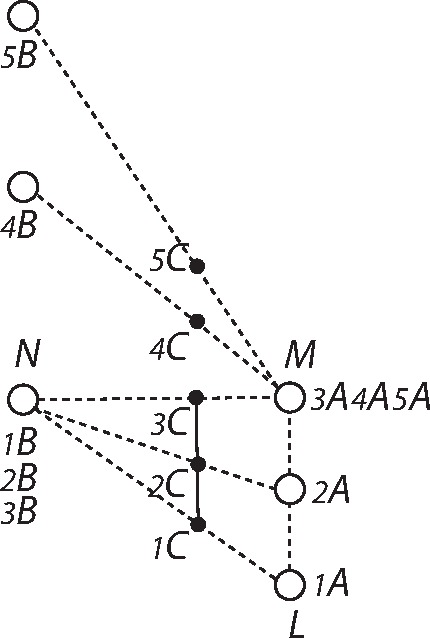
\includegraphics[width=0.3\textwidth]{%
gesamttex/edit_VIII,3/images/LH_37_05_017_d1.pdf%
}} 
\vspace{0.5em}
\centerline{%
\lbrack\textit{Fig.~1}\rbrack%
}
% \newpage%
\vspace{1.5em}
%
\pstart
\edtext{Ponatur}{%
\lemma{\hspace*{1,6mm}%
\lbrack\textit{Fig.~1}\rbrack%
}\killnumber%
\Cfootnote{%
Ein gestrichener Entwurf zum Diagramm wird nicht wiedergegeben.%
}}
%
in 
%
\edtext{\textit{{\scriptsize3}A} (\protect\vphantom)ubi}{%
\lemma{\textit{{\scriptsize3}A}}%
\Bfootnote{%
\textit{(1)}~jam quiesce %
\textit{(2)}~(\protect\vphantom)ubi~\textit{L}%
}}
%
minima est distantia a \textit{B}\protect\vphantom() 
%
jam quiescere corpus \textit{A} et moveri corpus \textit{B}. 
%
\edtext{Erit \textit{{\scriptsize3}C}\textit{{\scriptsize5}C}}{%
\lemma{Erit}%
\Bfootnote{%
\textit{(1)}~via %
\textit{(2)}~\textit{{\scriptsize3}C}\textit{{\scriptsize5}C}~\textit{L}%
}}
%
celeritas et via centri\protect\index{Sachverzeichnis}{via centri} eadem quae ante; sed 
%
\textit{{\scriptsize3}B}\textit{{\scriptsize5}B} celeritas ipsius \textit{B} est ad 
%
\textit{{\scriptsize3}C}\textit{{\scriptsize5}C}
%
\edtext{vel ad \textit{{\scriptsize1}C}\textit{{\scriptsize3}C}}{%
\lemma{}%
\Bfootnote{%
vel ad \textit{{\scriptsize1}C}\textit{{\scriptsize3}C} %
\textit{erg.~L}%
}}
%
ut $A+B$ ad \textit{B}. Ergo velocitas ipsius \textit{B} nempe \textit{{\scriptsize3}B}\textit{{\scriptsize5}B}
%
est ad velocitatem ipsius \textit{A} nempe \textit{{\scriptsize1}A}\textit{{\scriptsize3}A}, 
%
in composita ratione $A+B$ ad \textit{B}, et \textit{A} ad $A+B$ id est ut \textit{A} 
%
%
\edlabel{37_05_017_1a}%
\edtext{}{% NEUER ABSATZ UND VARIANTEN – "ad  B. Ergo"
{\xxref%
{37_05_017_1a}{37_05_017_1b}}%
\lemma{ad \textit{B}.}%
\Bfootnote{\textit{(1)}~Jam ipsius \textit{(2)}~Ergo \textit{(a)}~potentia \textit{(b)}~celeritate ipsius \textit{A} moti existente \textit{(aa)}~\textit{Avv} \textit{(bb)}~\textit{v} et potentia \textit{Avv}, erit \textit{(aaa)}~potentia \textit{(bbb)}~ipsius \textit{B} celeritas~\textit{L}}}%
ad \textit{B}.
\pend
%
\pstart
Ergo celeritate ipsius \textit{A} moti existente \textit{v} et potentia\protect\index{Sachverzeichnis}{potentia} \textit{Avv}, erit ipsius \textit{B} celeritas%
\edlabel{37_05_017_1b}
%
$Av:B$ et potentia $BAAvv:BB$ seu $AAvv:B$. Ergo non potest esse eadem quae ante.
\pend
%
\vspace{2.0em} %%%%%%%%% Diagramm 2
\centerline{%
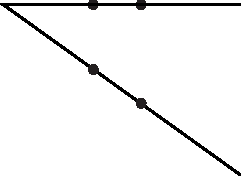
\includegraphics[width=0.22\textwidth]{%
gesamttex/edit_VIII,3/images/LH_37_05_017_d2.pdf%
}} 
\vspace{0.5em}
\centerline{%
\lbrack\textit{Fig.~2}\rbrack%
}%
\count\Afootins=1200%
\count\Bfootins=1200%
\count\Cfootins=1200